\documentclass[]{report}
\usepackage{tikz}
\newcommand{\inputtikz}[2]{%  
	\scalebox{#1}{\input{#2}}  
}

\usepackage{listings}
\usepackage{color}
\usepackage{amsmath}
\usepackage{mathtools}
\usepackage{graphicx}
\usepackage{caption}
\definecolor{dkgreen}{rgb}{0,0.6,0}
\definecolor{gray}{rgb}{0.5,0.5,0.5}
\definecolor{mauve}{rgb}{0.58,0,0.82}
%opening
\title{SY19}
\author{}

\begin{document}
	
\lstset{frame=tb,
	language=R,
	aboveskip=3mm,
	belowskip=3mm,
	showstringspaces=false,
	framexleftmargin=5mm,
	columns= fixed,
	numbers = left,
	basicstyle={\small\ttfamily},	
	numberstyle=\tiny\color{gray},
	keywordstyle=\color{blue},
	commentstyle=\color{dkgreen},
	stringstyle=\color{mauve},
	breaklines=true,
	breakatwhitespace=true,
	tabsize=3
}

\maketitle

\part{Abreviations}
\begin{tabular}{l r}
	MSE & Mean Squared Error \\
	RSE & Resiual Standard Error\\ 
	RSS & Residual \\
	R & \\
	BIC \\
	LR & Linear Regression \\
	CV & Cross Validation \\
	LOOCV & Leave One Out Cross Validation \\
	
\end{tabular}
\begin{abstract}

\end{abstract}

\chapter{Introduction}

\chapter{Ex 1}

\chapter{Ex 2 - Breast Cancer Recurring Time}

\section{Introduction}
This part aims to build the best model to predict the recurring time of breast cancer based on about 30 features computed from a breast mass.  This regression problem will take advantage of a given dataset describing about 200 patient cases.

\section{Dataset Description}
The very first step of our method consists in taking a look at the raw dataset to get precious hints on how each feature contributes to the recurring time. The dataset comprises 194 patient cases, each of which is described through 32 features and the cancer recurring time \texttt{Time} that we have to predict.

\subsection{Time}
Let's first describe the distribution of the variable \texttt{Time}. To do so, we can use the R functions \texttt{boxplot} (figure \ref{fig:time_boxplot}) and \texttt{hist} (figure \ref{fig:time_hist}). According to these figures, our dataset mostly represent short reapparing times.

\begin{figure}[!hb]
	\centering
	\inputtikz{0.5}{Figures/time_boxplot.tex}
	\caption{Box Plot}
	\label{fig:time_boxplot}
\end{figure}

\begin{figure}[!h]
	\centering
	\inputtikz{0.5}{Figures/time_hist.tex}
	\caption{Histogram}
	\label{fig:time_hist}
\end{figure}


\subsection{Features Description}
Each patient is represented with a set of 32 features extracted and computed from a digitized image of a breast mass. The data description we were given does not specify the units, but we do not need them for the following analysis.

Here are the 32 features we are provided with:  
\begin{itemize}
	\item Lymph Node Status
	
	\item Mean, Standard Error and Mean of the three largest values (also called "Worst") of 
		\begin{itemize}
			\item radius
			\item texture
			\item perimeter
			\item area
			\item smoothness
			\item compactness
			\item concavity
			\item concave points
			\item symmetry
			\item fractal dimension
		\end{itemize}
	
	\item Tumor Size
\end{itemize}

\subsubsection{Feature Correlation}
Based on the definition of the parameters described above, we already know that many features are correlated :
\begin{itemize}
	\item The mean of each parameters is smaller than the "worst" value;
	\item The radius, the perimeter and the area are most likely to be linked together;
	\item The compactness can be computed with the perimeter and the area thanks to the given formula : $Compactness = \frac{perimeter^2}{area - 1}$
\end{itemize}

\subsection{Data Relevance}
We should first check that every patient is relevant to our study, in other words, that there is no abnormal observation in the dataset. Cook's Distance is an interesting measure to verify this important criteria, it can be computed after a simple Linear Regression.

Cook's distance aims to study the influence of each observation on the regression coefficient estimates. To do so, this method uses a straight-forward approach that consists in computing the difference between the original coefficient estimates $\hat{\beta}$ and the coefficient estimates without taking into account the $i$-th observation $\hat{\beta}_{(-i)}$. The difference is then normalized using the number of parameters and the standard deviation estimate. 

A value higher than 1 often indicates an outlier that should be removed from the dataset.

In R, we can use the following code to compute and plot the Cook's distance of each observation :

\begin{lstlisting}
linreg = lm(Time ~ ., data=data_set)
cooks.distance(linreg)
\end{lstlisting} 

\begin{figure}[!h]
	\centering
	\inputtikz{0.5}{Figures/cooks_distance.tex}
	\caption{Cook's Distance}
	\label{fig:cook_distance}
\end{figure}

According to plot (figure \ref{fig:cook_distance}), no observation is located beyond the critical Cook's boundary of 1. This means that we can potentially use each and every patient case of our dataset to build our regression model. 

\subsection{Relation between "feature" and "time"}
In this section, we will take a first look at the relationship between the variable \texttt{Time} and the features used to describe a patient case. 

A first way to do it is to separately plot each relationship. An example of such plot is shown in figure \ref{fig:time_feature_ex1}. 

\begin{figure}[!h]
	\centering
	\inputtikz{0.5}{Figures/time_feature_ex1.tex}
	\caption{Plot of \texttt{Time} and \texttt{Texture Mean} }
	\label{fig:time_feature_ex1}
\end{figure}

Unfortunately, most plots show very scattered points that do not seem to follow any specific model. The variance is so significant that we cannot even estimate the type of function that links a feature and the variable \texttt{Time} together. It could be a simple linear model with a high variance that we may be able to estimate, or more complex models with non-linearities and feature correlations.

To have better clues on the type of model we should be dealing with, we can draw a QQ-Plot that plots the Studentized Residuals with the quantiles. 

In R, we can use the library \texttt{car} to easily draw the QQ-Plot (figure \ref{fig:qq_plot}) :
\begin{lstlisting}
library(car)
qqPlot(linreg, main="QQ Plot")
\end{lstlisting}

\begin{figure}[!hb]
	\centering
	\inputtikz{0.5}{Figures/qq_plot.tex}
	\caption{QQ-Plot}
	\label{fig:qq_plot}
\end{figure}

The bottom tail of the QQ-Plot seems to deviate from the linear line, which is a sign of the error's non-normality. This may mean that the error does not follow a normal model, or that the model is actually non-linear.

\begin{figure}[!hb]
	\centering
	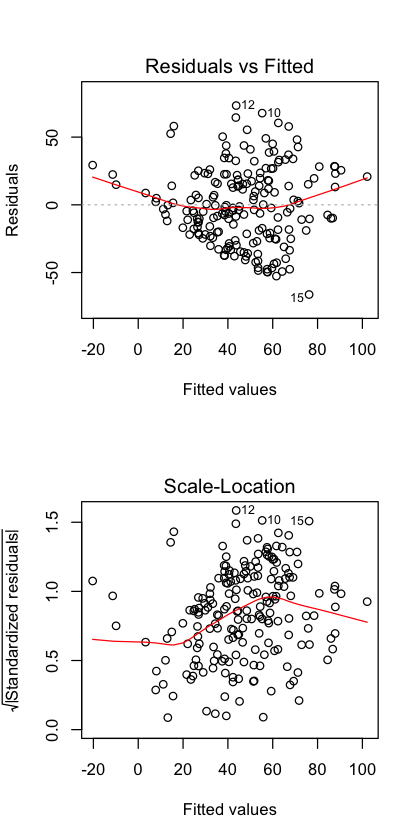
\includegraphics[width=0.5\linewidth]{Figures/fitted_value_plots}
	\caption{}
	\label{fig:fitted_value_plots}
\end{figure}

We can also analyze the Residuals-Fitted plot and the Scale-Location plot to get a better understanding on the model. To do, we can simply apply the function \texttt{plot} on the linear model (figure \ref{fig:fitted_value_plots}).

It turns out that both plots show non-normal scatters of the residuals. In particular, the points displayed in the Residuals-Fitted plot seem to follow a fan shape. This is a sign of a non-constant variance, also called heteroscedasticity.

\section{Measures to Compare Models}
Before building any model, we have to properly define the measures we will later use to compare them. 

\subsection{Some Measures}
A first way to assess the performance of a model is to compute the Mean Squared Error (MSE). We can also use adjusted $R^2$ score.

\subsection{Data Split}
These measures should not be applied on a set whose data was also used to train the model. Indeed, this would include a biais that might distort our conclusions. To cope with this problem, we have to split the dataset into two disjointed sets : 
\begin{itemize}
	\item Training Set : About 66\% of the dataset dedicated to the building the model;
	\item Test Set : The remaining 34\% only used at the end to provide some kind of objective measure of the model performance.
\end{itemize} 

\begin{lstlisting}
n = dim(data_set)[1]
train_id = sample(1:n, n * 2/3)

train_set = data_set[train_id,]
train_set.x = train_set[,-33]
train_set.y = train_set[,33]

test_set = data_set[-train_id,]
test_set.x = test_set[,-33]
test_set.y = test_set[,33]
\end{lstlisting}

Once it is done, we can finally dive into the model building.

\section{K-nearest neighbors (KNN)}
We start our analysis with a very simple model called the KNN.
Given a positive integer $k$ and a test observation $x_0$. The KNN model first identifies the k closest points to $x_0$ from the training data. Then estimates \\ 

\subsection{Knn Model}
The KNN model in R is done by calling the function \texttt{reg} of the package \texttt{knn}. As we will see in the following sections, For most prediction algorithms, we first have to build the prediction model on the training data, and then use the model to test our predictions. However, the KNN function does both in a single step.\\ 
In order to find the best $k$ we set a maximum number of neighbors to be considered (in our model it is 120), then we calculate the MSE for each $k$ which is the mean of the squared difference between the real value of Time and the predicted one. All the steps are detailed in the code below.

\subsubsection{Model Implementation}
\begin{lstlisting}
library(FNN)
k_max = 120;
MSE = rep(0,k_max)

for( k in 1:k_max)
{
	reg = knn.reg(train=cancer.train.x, test=cancer.test.x, y=cancer.train.y, k=k)
	MSE[k] = mean((cancer.test.y - reg$pred)^2)
}

plot(1:k_max, MSE, xlab='k', ylab='MSE', main='MSE against k neighbours')
points(x = best_k_test, y = best_k_mse, col = "red", pch = 16)
abline(h = best_k_mse, col='red')
abline(v = best_k_test, col='red')

best_k_test = which.min(MSE)
best_k_mse = MSE[best_k_test]
\end{lstlisting}

The graph below shows the MSE plotted against the values of $k$ in a range from 0 to 120. Graphically we notice that a minimum is reached between 10 and 20.

\begin{center}	
		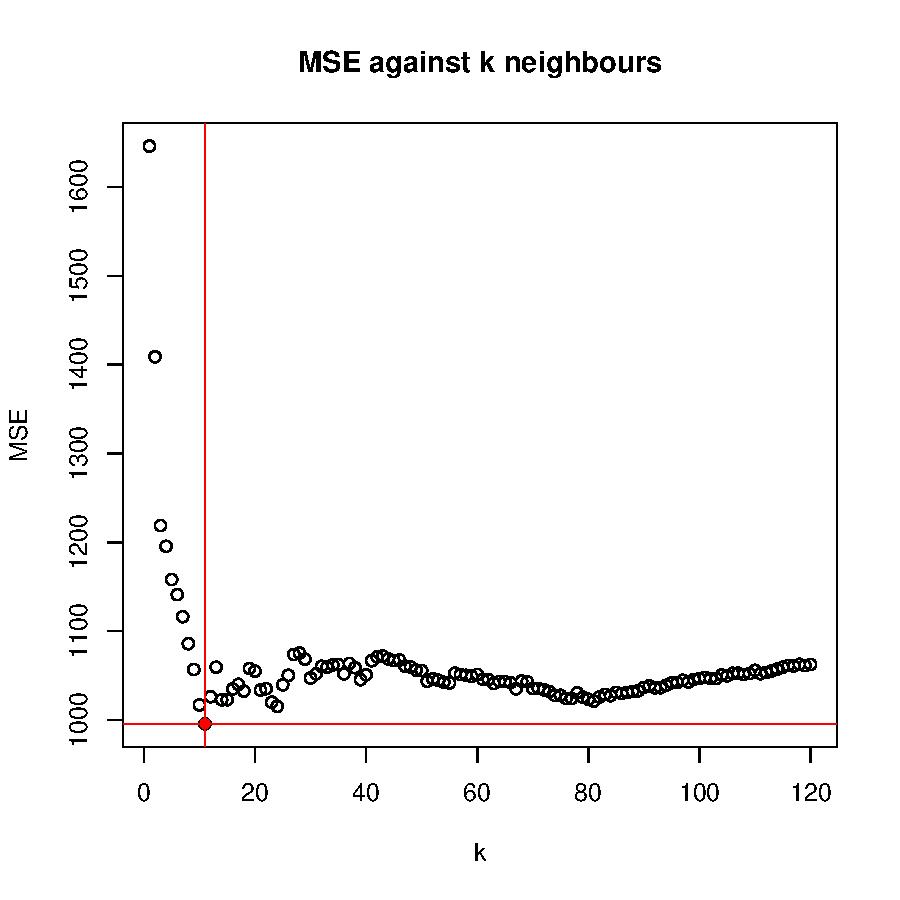
\includegraphics{Figures/knn_test.pdf}
		\captionof{figure}{MSE against K neighbours}
\end{center}

 We use the function \texttt{which.min} that returns the index of the minimum MSE value.\\

\begin{center} 
	best\_k\_test= 11 \\
	best\_k\_test\_MSE = 995.433185
\end{center}

Now that we have the k that minimizes the MSE we call KNN algorithm with this best k and plot the predicted values against the real values. The figure above shows the result.

\begin{lstlisting}
best_reg_test = knn.reg(train= cancer.train.x, test = cancer.test.x, y=cancer.train.y, k = best_k_test)
plot(cancer.test.y, best_reg_test$pred, xlab='y', ylab='y-hat', main='y-hat (Predicted) against y')
abline(0,1, col='red')
\end{lstlisting}

The red line is the function $y=x$; so further are the points from this line the further are the predicted values ($\hat{y}$) from the real one ($y$).
	
\begin{center}
	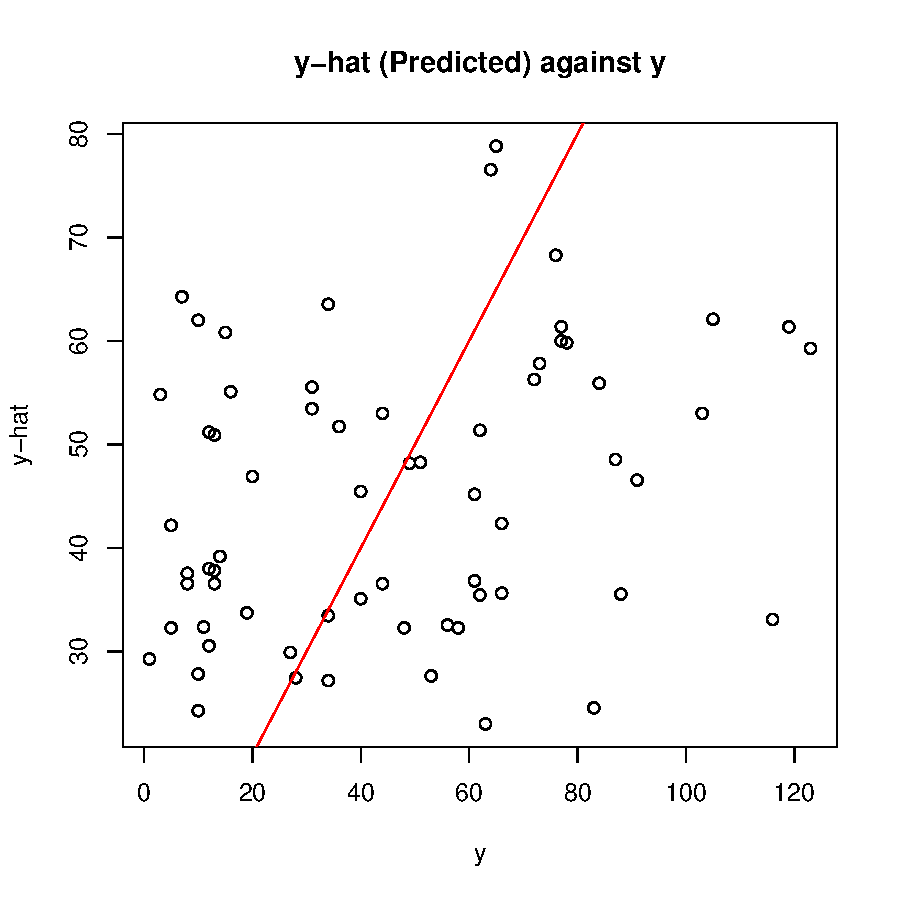
\includegraphics{Figures/knn_predicted_test.pdf}
	\captionof{figure}{MSE against K neighbours}
\end{center}

\subsubsection{Model Analysis}

We notice that the predicted {$\hat{y}$} diverge a lot the real values $y$. We expected those results since the MSE=967.386966 which is quite high. 

This approach of finding the best $k$ was quite optimistic. Actually we tried finding the best $k$ while minimizing the MSE in \textbf{the test data}. Therefore the model is very specific to our test data which yields to a high bias. The solution is to find the best $k$ among the \textbf{training data} and then use the best $k$ in the test data. \\ To find the best \textbf{unbiased} $k$ number of neighbors we use the method of cross validation on the train data. 

\subsection{The Validation Set Approach}
There are two methods in cross validation: \textbf{cross validation leave one out} and  \textbf{K-fold cross validation}. In the following parts we will test with both validation methods. As we do not have that much predictors we can afford the computation of cross validation leave one out.\\

\subsubsection{Cross Validation}
The cross validation approach is based on dividing the provided data in 2 sets: a training set and a validation set. The model is fit on the training set, then the fitted model is used to predict responses of observations in the validation set. The resulting validation set error rate is assessed using MSE.

\subsubsection{Leave-One-Out Cross-Validation}
Like the cross validation the LOOCV involves splitting the set of observations in two parts. The test data has a single observation $(x_1, y_1)$ and the $n-1$ remaining is used for the training data. The MSE in this case is $MSE_1 =(y_1 - \hat{y})^{2}$. This provides an unbiased estimate for the test error since it is training the model on approximately all the data of the observation. However it is highly variable as it is based in one observation. The LOOCV repeats the procedure n times fitting each time a different set of observations. The LOOCV test MSE is computed with calculating the average of the n test error estimates.
  
\begin{center}
	$$CV_{(n)} = \frac{1}{n} \sum_{i=1}^{n} MSE_{i} $$
\end{center}

The LOOCV will always give the same results in contrast to the CV that depends on the randomness of how the data are split. Furthermore the CV runs the training approach on around the half of the size of the original data while the LOOCV repeats the validation set approach n times using n-1 observations. Hence the LOOCV yields to a not overestimated test error rate compared to the validation. Nevertheless the disadvantaged of the LOOCV is it can be very time consuming when n the number of observations is large.\\

An alternative to LOOCV that has a smaller computation time is k-Fold Cross Validation. This approach based on dividing the training observations on k groups, each time one group will be considered as the test set and the k-1 left as the training set. Therefore the CV becomes:

\begin{center}
	$$CV_{(k)} = \frac{1}{k} \sum_{i=1}^{k} MSE_{i} $$
\end{center}

We can see that the k-Fold Cross-Validation fits the model k times instead of n, which reduces considerably the computation time. Our original data have 198 observations so we can afford the computation of the LOOCV. \\

\subsubsection{Model implementation}

\begin{lstlisting}
library("kknn")
model_kknn = train.kknn(Time ~., data= cancer.train, kmax = 30, ks = NULL, distance = 2, kernel = "optimal")
best_k_train = model_kknn$best.parameters$k
\end{lstlisting}

After deducting the best k neighbors from the model we use it on the test observations to predict the values of Time. 
We then compute the MSE and plot the predicted values $\hat{y}$ on the real ones \textit{y}.

\begin{lstlisting}
best_reg_train = knn.reg(train= cancer.train.x, test = cancer.test.x, y=cancer.train.y, k = best_k_train)
plot(cancer.test.y, best_reg_train$pred, xlab='y', ylab='prediction')
abline(0,1, col='red')
errors = (cancer.test.y - best_reg_train$pred)^2
mse= mean(errors)
\end{lstlisting}

The results are shown below:

\begin{center}
	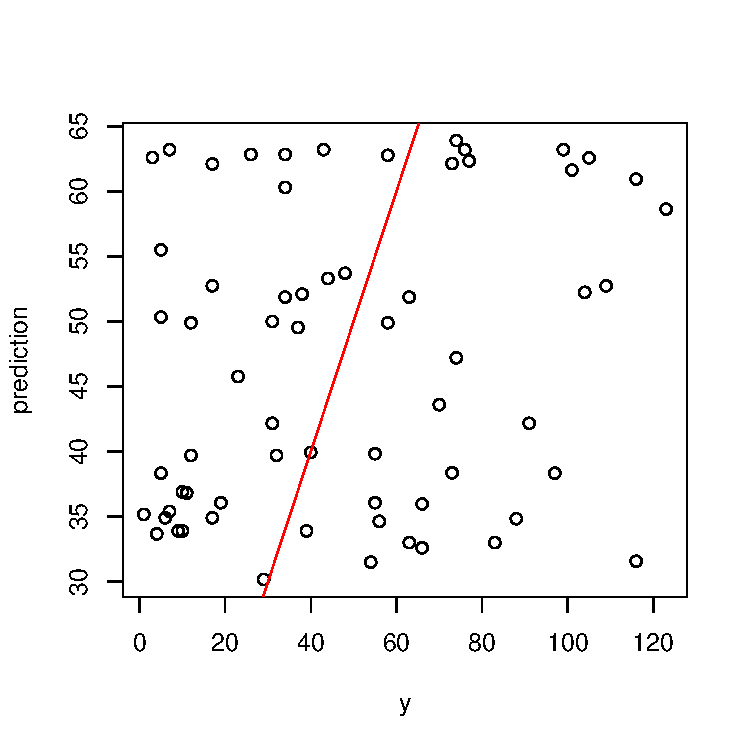
\includegraphics{Figures/knn_predicted_LOOCV.pdf}
	\captionof{figure}{MSE against K neighbours}
\end{center}

\begin{center} 
	best\_k\_train= 30 \\
	best\_k\_test\_MSE = 1047.085675
\end{center}

\subsubsection{Model Analysis}
One can argue that the prediction is not better since the test MSE obtained is higher that the one we had when we computed with the best test $k$. However the model with the validation approach is not biased, in other words, in general the $k=30$ will guarantee a smaller MSE than the $k=11$ on any test observation.

\section{Simple Linear Regression}
\subsection{Idea}
Our next attempt consists in using the same linear model we used in the feature analysis section. This model takes advantage of the simple assumption that \texttt{Time} depends on the other features in a linear way.

The model has the following form :
$$
	Y = \beta_0 + \sum_{i = 1}^{p} \beta_i X_i
$$
The regression coefficient $\beta_i$ are choosen so that they minimize the MSE. 

To build the model in R, we can use the function \texttt{lm} :
\begin{lstlisting}
model.linreg = lm(Time ~ ., data=train_set)
\end{lstlisting}

\subsection{Model Performance}
The MSE of this model is approximatively equal to 1285. The raw residuals distribution is pictured on figure \ref{fig:linreg_hist}, it shows a very spread out distribution that should be improved.

\begin{figure}[!h]
	\centering
	\inputtikz{0.5}{Figures/linreg_hist.tex}
	\caption{}
	\label{fig:linreg_hist}
\end{figure}

\section{Linear Regression with Features Selection}
\subsection{Idea}
A simple method to improve the performance of a simple Linear Regression is to select a subset of features that better describes the distribution of \texttt{Time}.

Once the simple linear model is fitted, we can use the function \texttt{summary} to display the value of each coefficient.
\begin{verbatim}
Coefficients:
Estimate Std. Error t value Pr(>|t|)  
(Intercept)              5.722e+01  1.587e+02   0.361   0.7191  
Lymph_node              -1.752e-01  7.034e-01  -0.249   0.8038  
radius_mean              3.001e+01  4.445e+01   0.675   0.5012  
texture_mean            -3.913e-01  2.043e+00  -0.192   0.8485  
perimeter_mean          -3.794e+00  6.651e+00  -0.570   0.5697  
area_mean               -1.328e-01  1.354e-01  -0.981   0.3291  
smoothness_mean         -7.124e+02  9.050e+02  -0.787   0.4331  
compactness_mean        -8.767e+01  3.554e+02  -0.247   0.8057  
concavity_mean          -2.654e+02  2.728e+02  -0.973   0.3332  
concave_points_mean      1.236e+03  5.911e+02   2.090   0.0392 *
symmetry_mean           -3.199e+01  2.647e+02  -0.121   0.9041  
fractal_dimension_mean   1.818e+03  1.666e+03   1.091   0.2781  
radius_se               -2.897e+01  9.953e+01  -0.291   0.7716  
texture_se              -1.784e+00  1.246e+01  -0.143   0.8865  
perimeter_se             8.817e+00  1.289e+01   0.684   0.4955  
area_se                 -3.871e-01  4.212e-01  -0.919   0.3604  
smoothness_se            2.987e+03  2.535e+03   1.178   0.2415  
compactness_se           7.135e+02  7.864e+02   0.907   0.3665  
concavity_se             3.798e+02  7.170e+02   0.530   0.5975  
concave_points_se       -7.782e+02  1.450e+03  -0.537   0.5926  
symmetry_se             -1.239e+03  7.861e+02  -1.576   0.1182  
fractal_dimension_se    -5.979e+03  6.280e+03  -0.952   0.3434  
radius_worst             9.300e-01  1.367e+01   0.068   0.9459  
texture_worst           -1.307e+00  1.964e+00  -0.666   0.5072  
perimeter_worst         -1.026e+00  1.449e+00  -0.708   0.4805  
area_worst               8.705e-02  7.021e-02   1.240   0.2181  
smoothness_worst        -3.761e+02  4.088e+02  -0.920   0.3599  
compactness_worst       -7.031e+01  9.964e+01  -0.706   0.4821  
concavity_worst         -3.011e+01  7.311e+01  -0.412   0.6814  
concave_points_worst    -2.181e+02  2.345e+02  -0.930   0.3546  
symmetry_worst           1.586e+02  1.425e+02   1.113   0.2687  
fractal_dimension_worst  1.028e+03  7.100e+02   1.448   0.1509  
Tumor_size              -1.188e+00  1.915e+00  -0.620   0.5364  
\end{verbatim}

The last column contains the P-value of each coefficient, which is a measure to test the hypothesis that this particular coefficient is null. A P-value lower than 5\% allows us to conclude that the coefficient is not equal to zero. In our case, the feature \texttt{concavity\_points\_mean} is not null, but we cannot make such assumptions for the other parameters. Therefore, we are not able to select a subset of interesting features based on the P-values.

Our dataset contains a small set of features to deal with, therefore we can use an exhaustive feature subset selection algorithm. Such method build a linear model based on each subset and compute a performance score to compare them. 

We use the following function to fit the linear models :
\begin{lstlisting}
model.linreg.regsubsets = regsubsets(Time ~ ., data=train_set, method = "exhaustive", nvmax = 32)
\end{lstlisting}

Then the function \texttt{plot} to compare the models according to a given scale (in this case, the BIC measure). The result is shown on figure \ref{fig:subset_bic}.
\begin{lstlisting}
plot(model.linreg.regsubsets, scale="bic")	
\end{lstlisting}

\begin{figure}[!h]
	\centering
	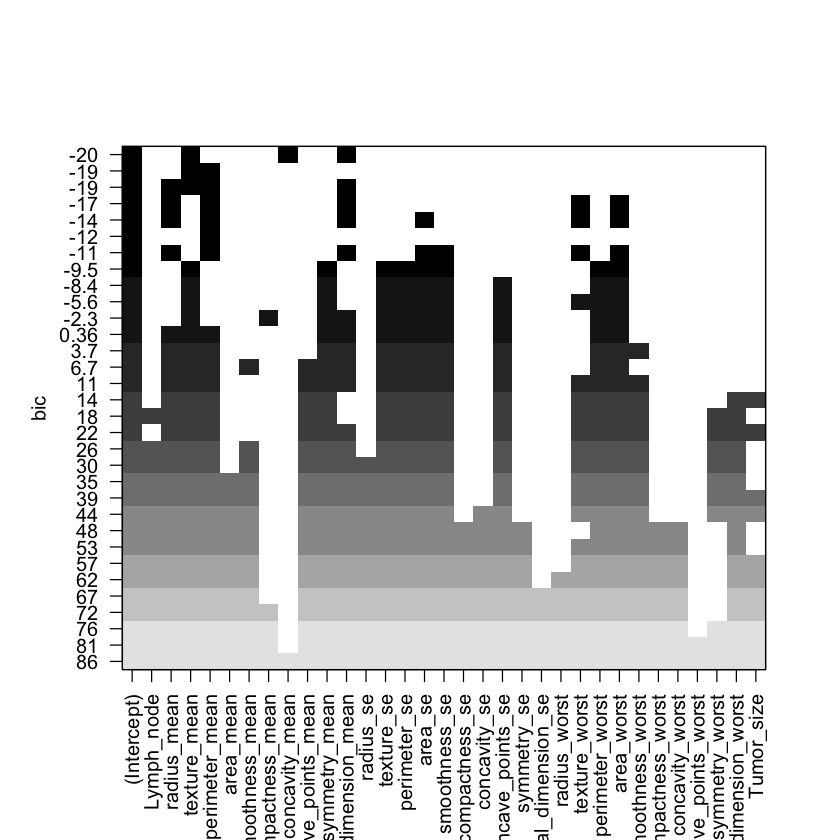
\includegraphics[width=0.8\linewidth]{Figures/subset_bic}
	\caption{}
	\label{fig:subset_bic}
\end{figure}

According to this plot, the best BIC is reached with a model that only uses the following features : 
\begin{itemize}
	\item \texttt{texture\_mean}
	\item \texttt{fractal\_dimension\_mean}
	\item \texttt{concavity\_mean}
\end{itemize}

\subsection{Model Performance}
The MSE of this model is approximatively equal to 1067. The raw residual distribution, shown on figure \ref{fig:subset_hist}, is way better than the simple linear regression model.

\begin{figure}[!h]
	\centering
	\inputtikz{0.5}{Figures/subset_hist.tex}

	\caption{}
	\label{fig:subset_hist}
\end{figure}

\section{Linear Regression with Regularization}
In this section we will discuss some methods that will help us shrink the model by reducing the number of parameters.
We will use the \textbf{glmnet} package in order to build the ridge regression and the lasso in R.

\subsection{Ridge Regression}
The Linear Regression with least squares estimates the parameters $\beta_{0},\beta_{1}...\beta_{p}$ that to minimize the term of the RSS.
\begin{center}
	$$ RSS = \sum_{i=1}^{n}(y_{i} - \beta_{0} - \sum_{j=1}^{p}\beta_{j}x_{ij})^{2} $$
\end{center}

Ridge Regression works the same way as the least squares in the sense that it also tries to minimize the RSS but is also has another term $\lambda \sum{j}\beta_{j}^{2}$ called the \textbf{shrinkage penalty} where $\lambda\geq$ 0 is the \textbf{ tuning parameter}. The formula is:
		\begin{equation} \label{eq1}
		  RSS + \lambda \sum_{j}\beta_{j}^{2}
		\end{equation}			

If $\lambda$=0 we are in the same case of a least squares estimates. The higher $\lambda$ gets, the higher will be the penalty. Hence Ridge regression will try to minimize the parameters $\beta_{j}$ in order to minimize the term \ref{eq1}.\\
\subsubsection{Model Implementation}
The \texttt{glmnet} function takes for parameters the matrix $x$ of predictors and vector $y$ of responses. The \texttt{model.matrix} will help us transform out data sets into matrix. This function not only gives out a matrix but it also converts the qualitative variables into dummy variables.
\begin{lstlisting}
x.train = model.matrix(Time~.,cancer.train)[,-1] 
y.train = cancer.train$Time

x.test =model.matrix(Time~.,cancer.test)[,-1]
y.test = cancer.test$Time
\end{lstlisting}
The glmnet function takes in parameter the train data, the pramater alpha that indicates whether it is a Ridge or Lasso regression that we want to perform (alpha=0 for Ridge). By default \texttt{glmnet} chooses an automatic range of $\kappa$, however here we chose a wide range $\lambda\in[10^{−2},10^{10}]$ to cover all possibilities.

\begin{lstlisting}
library(glmnet)
grid = 10^seq(10, -2, length=100)
ridge.mod = glmnet(x.train, y.train, alpha=0, lambda=grid)
plot(ridge.mod)
\end{lstlisting}

\begin{center}
	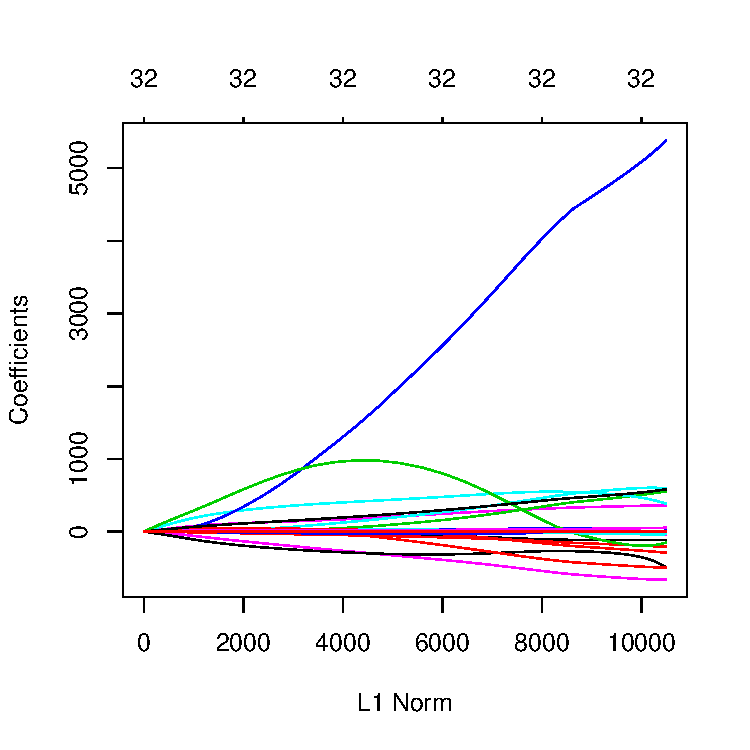
\includegraphics{Figures/ridge_model.pdf}
	\captionof{figure}{Coefficients $\beta_{j}$ against L1 Norm}
\end{center}

The figure below shows that the higher the norm L1 is the smaller are the coefficients $\beta_{j}$.\\

In order to find the best tuning parameter $\lambda$ we perform a cross validation on the training data. cv.glmnet function runs a 10 fold cross validation on the data.

\begin{lstlisting}
cv.out = cv.glmnet(x.train, y.train,alpha=0)
plot(cv.out)
best_lambda = cv.out$lambda.min
\end{lstlisting}

\begin{center}
	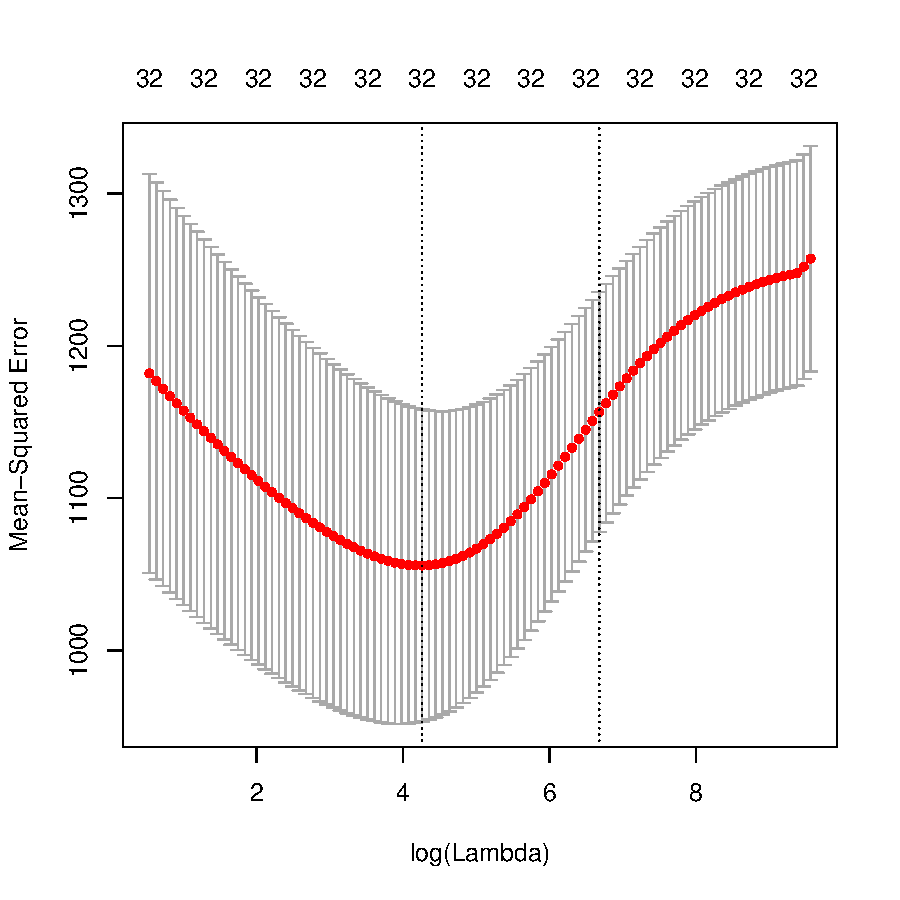
\includegraphics{Figures/cv_glmnet.pdf}
	\captionof{figure}{MSE against log($\lambda$)}
\end{center}

The value $\lambda$ that yields to the smallest MSE is shown in the graph near $log(\lambda)=4$ and $log(\lambda)=5 $


\begin{lstlisting}
fit.ridge = glmnet(x.train, y.train, lambda=best_lambda, alpha=0)
ridge.pred = predict(fit.ridge, s=best_lambda, newx=x.test)
MSE = mean((y.test - ridge.pred)^2)
residuals = y.test - ridge.pred
plot(x=y.test, y=ridge.pred)
abline(0,1, col='red')
plot(x=y.test,y=residuals)
\end{lstlisting}

\begin{center} 
	best\_$\lambda$ = 3.522385 \\
	best\_test\_MSE = 1017.18
\end{center} 

\begin{center}
	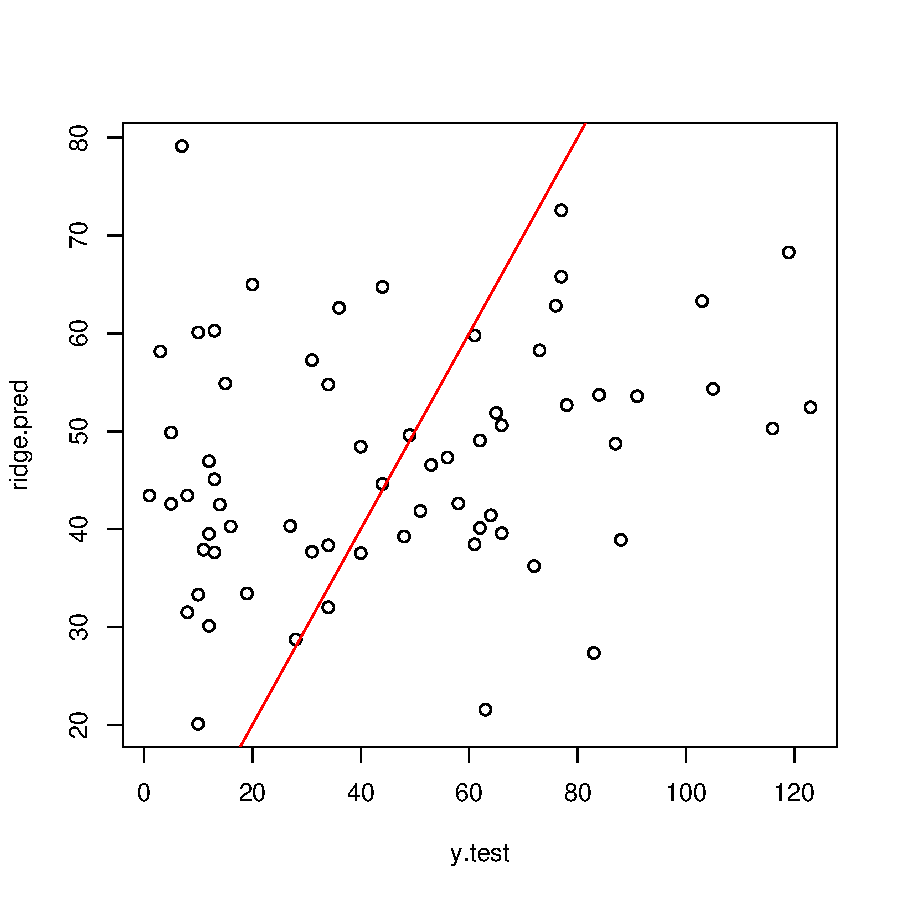
\includegraphics{Figures/ridge_yhat.pdf}
	\captionof{figure}{predicted Time $\hat{y}$ against real responses y }
\end{center}

\begin{center}
	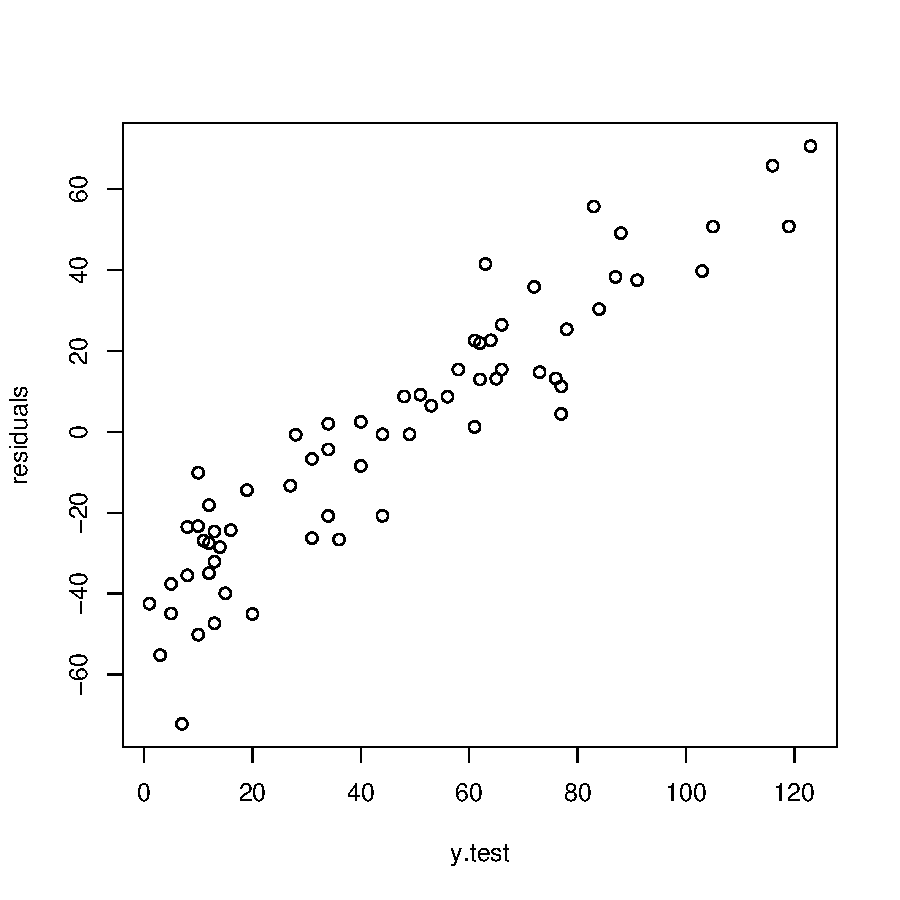
\includegraphics{Figures/ridge_resid.pdf}
	\captionof{figure}{Residuals against Time(y)}
\end{center}

Performing a Ridge regression didn't really improve out MSE, we notice that we still have the same shape when we plot the predicted response against the real values. In fact we still have the extreme values scattered away from the line y=x while the values in the middle are grouped around it. The residuals shows most residuals are among -20 and 40, however we can't neglect the important number of observation that have residuals below -20.\\

After predicting the responses with the best\_$\lambda$,  we can also to get the coefficients $\beta_{j}$ for this model.

\begin{lstlisting}
predict(ridge.mod, type="coefficients", s=best_lambda)[1:33,]
\end{lstlisting}

\begin{center}
	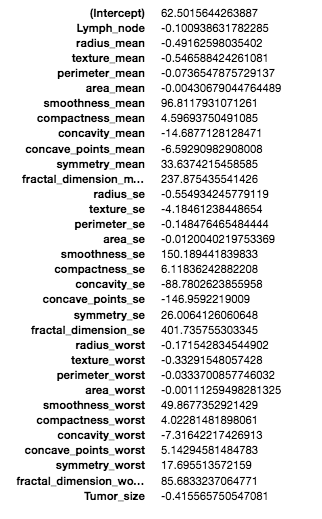
\includegraphics{Figures/ridge_coeff}
	\captionof{figure}{coefficients $\beta_{j}$ for ($\lambda$ = 64.48)}
\end{center}

\subsubsection{Model Analysis}
So we notice that some coefficients are very close to 0 such as \texttt{area\_se }(-0.012), but none of them is null. In fact Ridge Regression only shrinks the coefficients and does not perform any variable selection;  that is why we are going to use Lasso in the following part.

After comparing both MSE of the least squares and Ridge Regression we notice that Ridge did not really improve our prediction. The question is why do we still affirm that Ridge improves over the least squares? It all can be summarized in\textbf{ biais-variance trade-off}. Let's take the following example where we we fit the model for each $\lambda$ and predict the responses for $\lambda\in[10^{-1},10^{4}]$. For each value of $\lambda$ we compute the MSE, the squared bias and the cube root of the variance. We computed the cube root in order to be able to scale purposes.
\begin{lstlisting}
max = 100
biais2<-rep(0,Kmax)
variance<-rep(0,Kmax) 
mse<-rep(0,Kmax)
grid=10^seq(4,-1, length=max)
for( i in 1:max)
{     
	fit.ridge = glmnet(x.train, y.train, lambda=grid[i], alpha=0)
	ridge.pred = predict(fit.ridge, s=grid[i] ,newx=x.test)
	mse[i] = mean((ridge.pred - y.test)^2) #MSE
	biais2[i] = (mean(ridge.pred - y.test))^2 #squared bias
	variance[i] = (var(ridge.pred))^(1/3) #variance
}
plot(grid, variance,type='l', xlab="lambda", main="Biais-Variance trade-off")
lines(grid, biais2,col='red')
plot(mse)
\end{lstlisting}

\begin{center}
	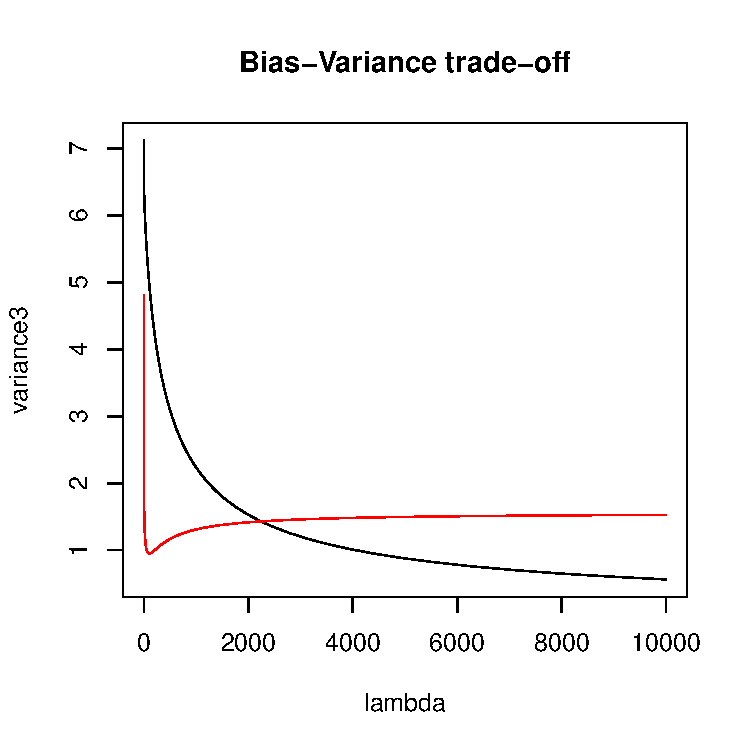
\includegraphics{Figures/ridge_biais_var.pdf}
	\captionof{figure}{Bias Variance trade-off, squared bias(red), root squared variance(black)}
\end{center}

\begin{center}
	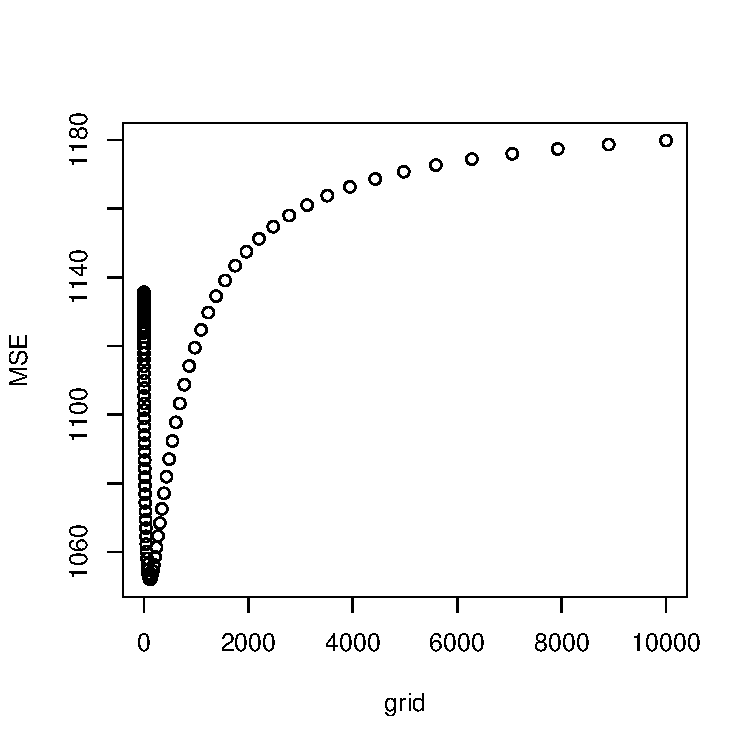
\includegraphics{Figures/ridge_mse.pdf}
	\captionof{figure}{MSE against $\lambda$}
\end{center}

At $\lambda=0$ (least squares), the variance is high but there is no bias.
As $\lambda$ increases the variance and bias decrease but at some point the variance continues to decrease while the bias starts increasing. Which means that the shrinkage of the coefficients by $\lambda$ reduces the variances on the expense of the bias, which can be explained by the fact that $\lambda$ in underestimating the coefficients by shrinking them. Let us compare now those results to the MSE curve. 
$$MSE = (E[\varTheta]-\varTheta)^{2} + Var(\varTheta) = (Bias[\varTheta])^{2} + Var(\varTheta)$$
Hence if the variance and the bias decrease significantly in the beginning the MSE will decrease too, and when the variance will decrease less and the bias will start increasing the MSE will increase too. We should also note that at at  $\lambda=0$ (least squares) the MSE is high.\\
To sum up, in linear regression we can have a low bias but a high variance, this is where the ridge regression improves over the least squares because it shrinks the variance on the expense of the bias.
  
\subsection{Lasso Regression}
As it was discussed on the previous section, Ridge regression disadvantage is that it does not perform a variable selection. Lasso Regression tries to minimize the term:

\begin{equation} \label{eq2}
	RSS + \lambda \sum_{j}{|\beta_{j}^{2}|}
\end{equation}	

The only difference with the term of Ridge is that now we have $|\beta_{j}^{2}|$ instead of $\beta_{j}^{2}$. This alternative will reduce the $\beta_{j}$ that are close to zero to null.
Hoping we have a more interpretable model with reducing the number of variables. To call the lasso model we use the same function glmnet but with alpha=1.
 
\subsubsection{Model Implementation}
\begin{lstlisting}
grid = 10^seq(10,-2, length=100)
lasso.mod = glmnet(x.train, y.train, alpha=1,lambda=grid)
plot(lasso.mod)
\end{lstlisting}

\begin{center}
	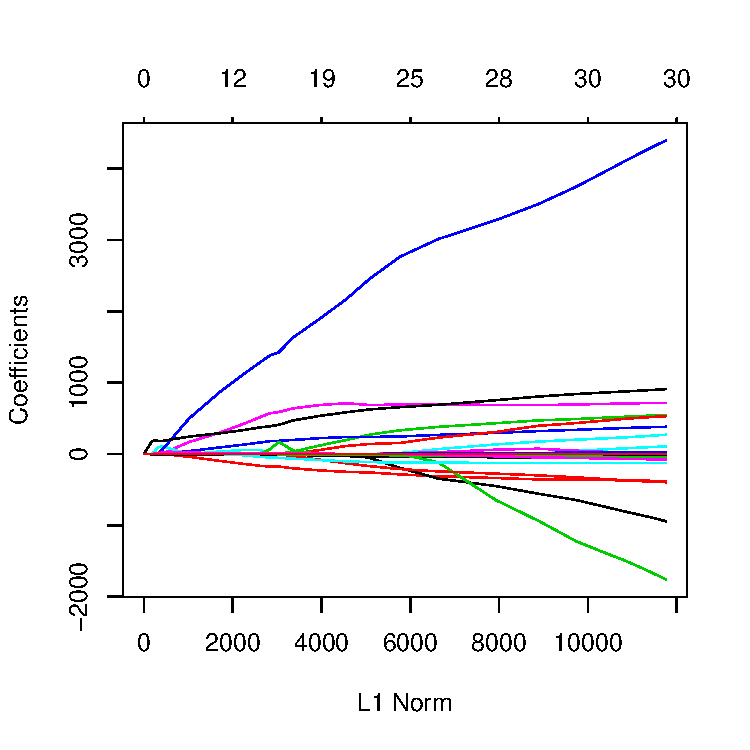
\includegraphics{Figures/lasso_coeff.pdf}
	\captionof{figure}{MSE against $\lambda$}
\end{center}

We notice that for some values of $\lambda$ the coefficients are null. We now perform the 10 fold cross validation on the training set to deduct the best tuning parameter.

\begin{lstlisting}
cv.out = cv.glmnet(x.train, y.train, alpha=1)
plot(cv.out)
best_lambda = cv.out$lambda.min 
lasso.pred = predict(lasso.mod, s=best_lambda , newx=x.test)
mean((lasso.pred-y.test)^2)
plot(x=y.test, y=lasso.pred)
abline(0,1, col='red')
\end{lstlisting}

\begin{center}
	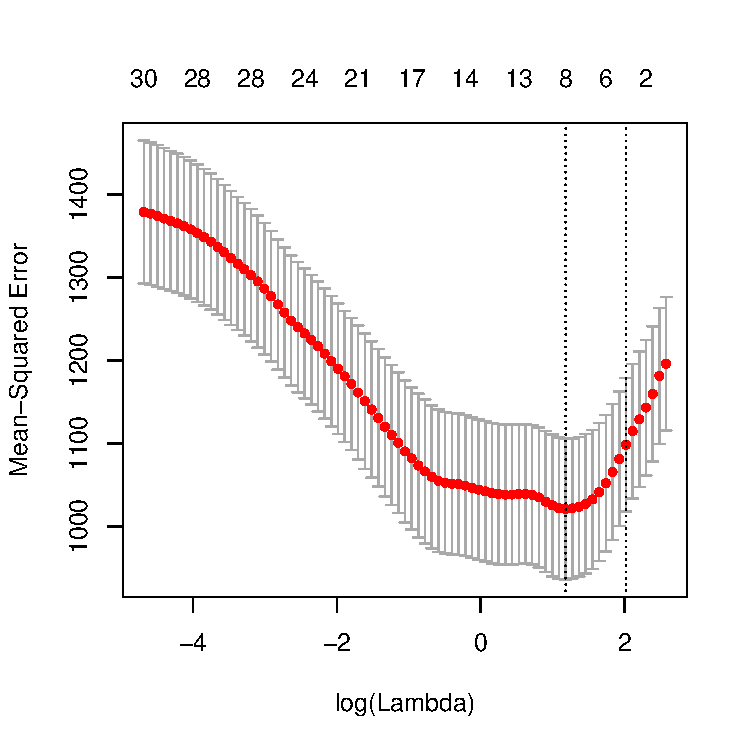
\includegraphics{Figures/lasso_mse.pdf}
	\captionof{figure}{MSE against $\lambda$}
\end{center}

\begin{center}
	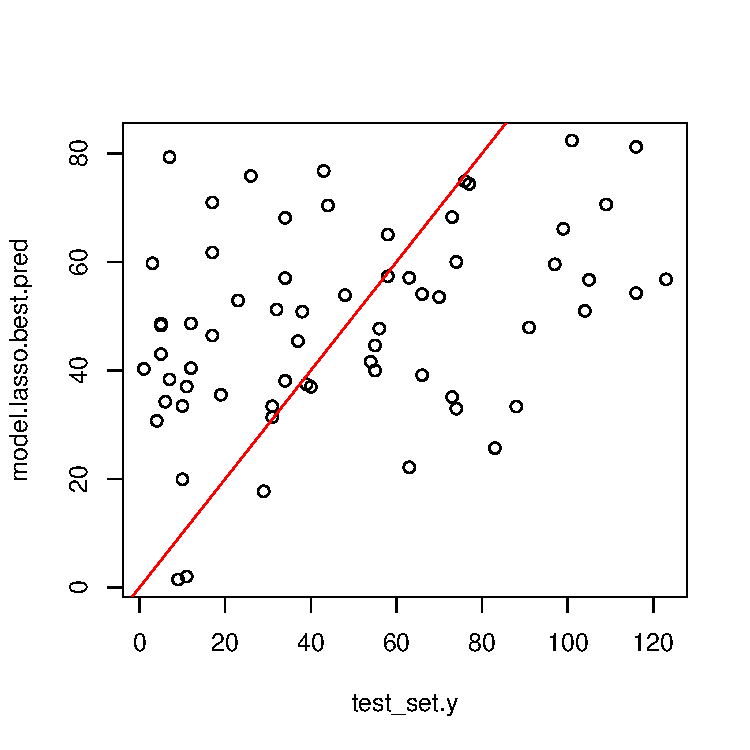
\includegraphics{Figures/lasso_predicted.pdf}
	\captionof{figure}{MSE against $\lambda$}
\end{center}

\begin{lstlisting}
predict(lasso.mod, type="coefficients", s=best_lambda)[1:33,]
\end{lstlisting}

\begin{center}
	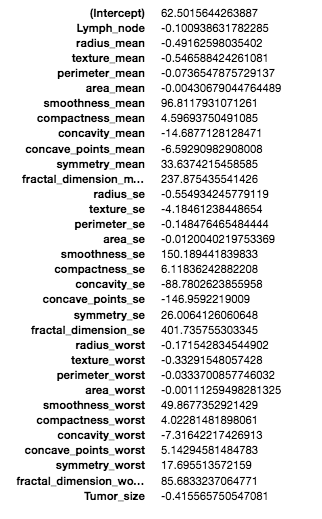
\includegraphics{Figures/ridge_coeff}
	\captionof{figure}{coefficients $\beta_{j}$ for ($\lambda$ = 64.48)}
\end{center}

We can clearly see that Lasso performed a variable selection by setting some coefficients to 0.

\subsubsection{Model Analysis}

\section{Linear Regression with Dimension Reduction}
\subsection{Idea}
In the Introduction, we mentionned the fact that some features are actually correlated. This means that they carry redundant information that make the model more complex, thus harder to fit. In this section, we will apply a Dimension Reduction method that decreases the number of features while keeping the information needed to predict \texttt{Time}.

Principal Component Analysis (PCA) is one such method. It consists in transforming the set of $p$ features into a set of $M$ orthogonal vectors ($M$ < $p$) using linear transformations. The new set of vectors (called components) contains as much information as the initial set. "Information" is here defined in terms of variance, in other words, each new component should be able to explain as much variance as possible, while being orthogonal to the others.

Once the set of principal components is found, it can be used as an input to a simple linear regression to build what is called a Principal Component Regression (PCR) model. The number of components $M$ should be taken so that the model built with PCR has a minimum error value; once again, a 10 fold cross validation method can be used to determine the best $M$.

PCR is available in R with the package \texttt{pls} :
\begin{lstlisting}
library(pls)
model.pcr = pcr(Time ~ ., data=train_set, scale=TRUE, validation="CV")
\end{lstlisting}

We can then plot the MSE for each set of components :
\begin{lstlisting}
validationplot(model.pcr, val.type = "MSEP")
\end{lstlisting}

According to figure \ref{fig:pcr_cv}, the model with only 4 components yields the best MSE. The function \texttt{summary} tells us that 4 components are enough to explain 75\% of the features' variance. 

\begin{figure}[!h]
	\centering
	\inputtikz{0.5}{Figures/pcr_cv.tex}
	\caption{PCR}
	\label{fig:pcr_cv}
\end{figure}



\section{Models Comparaison}

*USE TEST SET TO COMPARE MODEL*

\end{document}
